\chapter{Fundamentação Teórica}
\label{chap:cap2}

O presente capítulo apresenta os principais conceitos utilizados neste trabalho. A Seção \ref{sec:ambiente} introduz o ambiente RoboMind e a linguagem ROBO que é utilizada para programar os robôs virtuais dentro deste ambiente. Na Seção \ref{sec:verificacao} é explanado sobre a importância da verificação automática através da Verificação de Modelos e as principais técnicas utilizadas. Na Seção \ref{sec:csp} é introduzido sobre a especificação CSP e sobre a representação formal atual de ROBO, além de explicar como ocorre uma verificação na ferramenta FDR. Por fim, na Seção \ref{sec:compilacao} é explicado como ocorre o processo de compilação através da plataforma Spoofax.

\section{Ambiente RoboMind}
\label{sec:ambiente}
%Adicionar uns dois paragrafos sobre a simulação de robos

%\subsection{Ambiente RoboMind}

RoboMind\footnote[3]{http://robomind.net/} é um ambiente de programação de robôs virtuais para o ensino e aprendizagem de robótica. A Figura \ref{fig:robomind} ilustra a versão desktop deste ambiente que possui uma interface com um espaço para a escrita do programa que controla o robô virtual e um outro espaço onde o aluno pode acompanhar a execução (simulação) do robô em um mapa. Nesse ambiente, os programas são escritos na linguagem ROBO, uma linguagem educacional desenvolvida para a programação de robôs que oferece os principais comandos de programação: estruturas condicionais, estruturas de repetição, procedimentos e declaração de variáveis. O lado esquerdo da Figura \ref{fig:robomind} mostra um exemplo de programa ROBO que movimenta o robô enquanto o objeto (\texttt{beacon}) não é detectado à sua frente. Neste programa, se não há nenhum obstáculo à sua frente, o robô avança uma célula (comando \texttt{forward}), caso contrário o robô recua uma célula (comando \texttt{backward}) e muda sua orientação para a direita (comando \texttt{right}).

\begin{figure}[ht]
\centering
\caption{RoboMind, ambiente de programação de robôs virtuais}
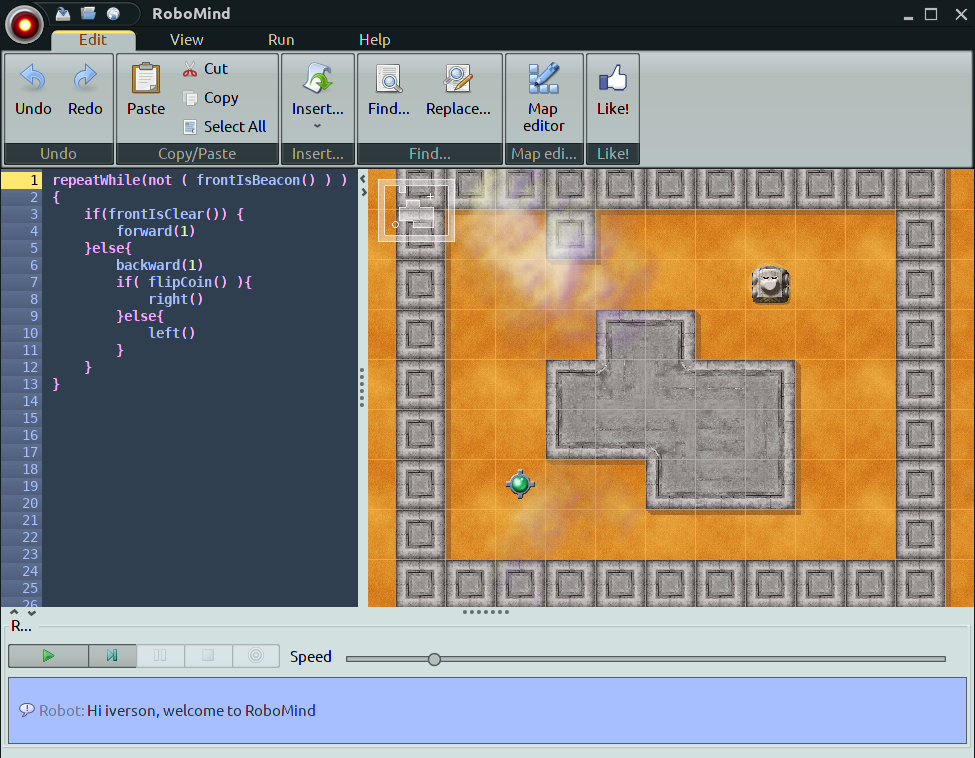
\includegraphics[height=10cm]{figuras/robomind_ide3.png}
\fonte{O autor}
\label{fig:robomind}
\end{figure}

%\subsection{Linguagem ROBO}

A seguir, listamos as principais construções sintáticas da linguagem ROBO.

\begin{itemize}
    \item Funções booleanas predefinidas para detecção de obstáculos e objetos ao redor do robô, por exemplo, a função \texttt{frontIsObstacle} retorna verdadeiro quando há um obstáculo na frente do robô (retorna falso no caso contrário), e a função \texttt{frontIsClear} retorna verdadeiro quando a frente do robô está livre de quaisquer objetos (retorna falso no caso contrário).
    \item Comandos predefinidos para movimentar o robô, como por exemplo o comando \texttt{forward(n)} que movimenta o robô para frente \texttt{n} células no mapa, e o comando \texttt{backward(n)} que movimenta o robô para trás \texttt{n} células.
    \item Comandos para a mudar a orientação do robô, como por exemplo o comando \texttt{right} que é usado para alterar a orientação do robô para a direita, e o comando \texttt{left} que é usado para alterar a orientação do robô para esquerda.
    \item Estruturas condicionais e de repetição, como por exemplo, \texttt{if-else}, \texttt{repeat(n)} e \texttt{repeatWhile}.
    \item Possui o procedimento \texttt{show(v)} que exibe o valor de uma expressão inteira ou booleana \texttt{v} recebida como parâmetro.
    \item Permite definir variáveis globais que armazenam valores inteiros ou booleanos.
    \item Permite que o usuário defina procedimentos parametrizados e não parametrizados.
\end{itemize}

Para exemplificar a abordagem de tradução, introduzimos um exemplo de programa em ROBO que conta a quantidade de caixas em um mapa. Este exemplo é uma adaptação do problema ``Contando Caixas'' proposto em RoboLab-FURB \cite{furb}. O objetivo desse exemplo é fazer com que o robô seja capaz de contar caixas dispostas na primeira ou na última linha de um mapa com três linhas.  A Figura \ref{fig:map} mostra um possível mapa utilizado usado como entrada para o programa que conta as caixas. Nele é possível ver um robô e algumas caixas: duas caixas na linha superior e três na linha inferior. Na figura foi adicionado um ``X'' para indicar a posição final que o robô deverá parar após a execução do programa. 

\begin{figure}[h]
\centering
\caption{Exemplo de Mapa usado no RoboMind}
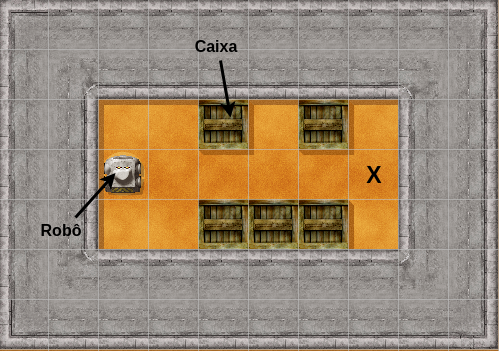
\includegraphics[height=7cm]{figuras/map2.png}
\fonte{O autor}
\label{fig:map}
\end{figure}

%Iverson: adicionei este paragrafo explicando sobre mapa no robomind
Um mapa no RoboMind é representado textualmente por um conjunto de letras para representar cada elemento do mapa. A Figura \ref{fig:maprobo} mostra a representação textual do mapa ilustrado na figura anterior. O carácter \texttt{@} representa o robô, as caixas são denotadas pela letra \texttt{Q} e as paredes pelos demais caracteres.

\begin{figure}[h]
\centering
\caption{Representação textual para um mapa do RoboMind}
\lstinputlisting[xleftmargin=4cm,xrightmargin=4cm]{codes/map.map}
\fonte{O autor}
\label{fig:maprobo}
\end{figure}

%\textbf{um parágrafo dizendo que não existe verificação automática de robôs educacionais. Motivar porque verificação de robôs é importante . Isto tem um pouco na introdução mas precisa colocar aqui novamente. Neste parágrafo aproveitar e dizer que verificação de modelos pode ajudar na verificação automática que é o assunto da próxima seção.}

Na literatura não há trabalhos que utilizem técnicas de verificação automática para programas objetivando a simulação de robôs educacionais. O que não garante que os programas foram escritos corretamente no contexto para o qual foram programados. Os próprios ambientes de programação não provém essa automaticidade, além da verificação sintática de código, por este motivo o aluno acaba verificando manualmente os programas. Por meio de técnicas automáticas é possível verificar diferentes propriedades de um programa e provar formalmente que estas propriedades são satisfeitas, como a ausência de \textit{deadlock} e outras propriedades específicas de um programa \cite{miyazawa}. Uma dessas técnicas é a Verificação de Modelos, descrita na seção seguinte.

\section{Verificação de Modelos}
\label{sec:verificacao}
O crescimento e a complexidade dos sistemas de software possibilita que falhas sejam empregadas durante o desenvolvimento, o que pode acarretar em prejuízos financeiros e desperdício. Quando o software consiste em um sistema crítico as perdas podem ser irreparáveis, como exemplo, perda de vidas humanas \cite{Clarke:1996}. Por essa razão, a Engenharia de Software vem propondo técnicas para auxiliar o processo de desenvolvimento de software, objetivando a construção de sistemas confiáveis para as mais diversas finalidades. Métodos formais~\cite{rui_silva} consistem em métodos da engenharia de software baseados em princípios matemáticos e apoiados por linguagens formais. Métodos formais são métodos rigorosos para a verificação de propriedades de sistemas, de modo a garantir que comportamentos indesejáveis não venham a acontecer~\cite{bhatt}.

Uma especificação formal é a base para vários métodos formais; consiste na descrição de um sistema e suas propriedades em uma linguagem formal. Essa especificação é a base para a verificação consistente das propriedades de um sistema~\cite{gannon,rui_silva}. A partir da especificação é possível explorar os possíveis estados alcançados por um sistema considerando um conjunto de entradas e saídas, afirmando, assim, as propriedades antes mesmo que o sistema seja implementado.

Na literatura de métodos formais, existem duas principais técnicas de verificação, a Verificação de Modelos (\textit{Model Checking}) e a Verificação Dedutiva (\textit{Deductive Verification}). A verificação formal tem sido gradualmente utilizada como um importante passo para a modelagem de sistemas críticos. Verificação de Modelos (\textit{Model Checking}) é uma das técnicas mais usadas dentro dos métodos formais; tem sido muito utilizada principalmente na verificação de sistemas concorrentes \cite{ZHAO2014}. Como estes verificadores proveem técnicas automáticas, sua utilização se torna muito efetiva para sistemas dessa finalidade.

%\subsection{Verificação de Modelos}

Apesar de pouco utilizada no contexto educacional, a verificação automática de programas pode ser utilizada para obter \textit{feedback} automático sobre o funcionamento dos programas. 

%A técnica Verificação de Modelos é uma coleção de métodos para a verificação formal automatizada de sistemas concorrentes.  
Verificação de modelos consiste em utilizar como entradas para uma ferramenta de verificação de modelo (\textit{Model Checker}) um modelo do sistema, que pode ser expressado usando álgebra de processos ou até notação UML (\textit{Unified Modeling Language}), como também a especificação das propriedades que o sistema deve satisfazer \cite{FEIGN}. A Verificação de Modelos automaticamente analisa exaustivamente que a especificação de um sistema satisfaz as propriedades definidas. Essa análise pode ser por meio de Lógica Temporal Linear (\textit{Linear Temporal Logic} - LTL) ou Lógica de Árvore de Computação (\textit{Computation Tree Logic} - CTL) \cite{ZHAO2014}. Como saída da verificação automática, temos o resultado positivo, se as propriedades são satisfeitas pelo modelo, ou resultado negativo, se as propriedades não são satisfeitas. Quando o resultado é negativo, o verificador de modelos mostra um cenário de execução onde o sistema não satisfaz alguma das propriedades, isso é chamado de contraexemplo. Uma desvantagem da Verificação de Modelos é que a técnica só consegue analisar sistemas com número finito e relativamente pequeno de estados. 

A técnica Verificação Dedutiva, diferentemente da Verificação de Modelos, é manual e requer maior conhecimento e experiência do usuário, entretanto, considera todos os estados possíveis do sistema, mesmo que sejam infinitos \cite{FEIGN}. Neste trabalho usamos Verificação de Modelos escritos na notação formal CSP para a verificação automática de programas escritos na linguagem robô.

\section{Modelo CSP para programas ROBO}
\label{sec:csp}
\textit{Communicatting Sequential Processes} (CSP) é uma álgebra de processos usada na especificação formal de sistemas concorrentes e distribuídos \cite{Cleaveland2018}. Essa notação é composta por processos e eventos que são utilizados para a especificação de um sistema. Eventos são uma abstração para ocorrência de ações do sistema ou do usuário como, por exemplo, os comandos de movimentação do robô podem ser modelados como eventos. Processos definem a ordem de ocorrência dos eventos \cite{Roscoe2010}. Na sintaxe de CSP, \texttt{P = e1 -> ... -> en -> Q} representa um processo \texttt{P} que comunica uma sequência de eventos \texttt{e$_i$}, separados pelo operador de prefixo de CSP (\texttt{->}) e se comporta como o processo \texttt{Q} após comunicar o último evento.

Os comandos e o ambiente de RoboMind foram modelados usando a notação de CSP em~\cite{nogueira}. O modelo CSP proposto permite representar os estados possíveis de um programa ROBO, considerando a execução dos comandos a partir da posição inicial do robô em uma mapa. Neste modelo, a posição do robô, sua orientação e a posição do \textit{beacon} são variáveis que são modificadas pela execução dos comandos contidos no programa do robô.

A Figura \ref{fig:model} mostra uma parte da especificação CSP usada para modelar um programa ROBO. A notação de CSP não possui variáveis. Uma forma de modelar variáveis em CSP é criando processos que funcionam como uma memória RAM, e canais que são usados para ler e atualizar as variáveis mantidas no processo memória. Na linha 4 estão definidos os canais (\texttt{channel}) \texttt{get} e \texttt{set}. O primeiro canal é uma abstração para a consulta de uma variável. O segundo representa uma atualização de uma variável. O tipo destes canais é \texttt{VarType}, expressado na linha 2. Este tipo contém o nome das variáveis do programa e as respectivas faixas de valores para as variáveis. A ferramenta que é utilizada para verificação (FDR) precisa que todos os valores a serem analisados tenham limite superior e inferior. Por exemplo, a variável \texttt{X} representa a coluna da posição atual do robô, os valores desta variável correspondem ao conjunto \texttt{TX}, cujos valores variam de 0 até a quantidade máxima de coluna de um mapa. A variável \texttt{Y} representa a linha da posição atual do robô, a variável \texttt{ORIENTATION} a orientação atual do robô. As variáveis \texttt{BX} e \texttt{BY} representam a posição do objeto \textit{beacon} (quando presente no mapa). Cada variável é guardada em uma célula de memória. A linha 6 apresenta o processo \texttt{Mcel(v,val)} que simula uma célula da memória, onde \texttt{v} é a variável e \texttt{val} o seu valor. Esse processo pode comunicar dois eventos: \texttt{get!v!val}, para comunicar o nome e o valor da variável; e \texttt{set!v?val\_}, para exibir o nome e um novo valor para a variável. Na linha 9, há o processo \texttt{Memory(binding)} com a finalidade de colocar as células de memória em paralelo. Este paralelismo é representado pelos símbolos \texttt{|||}, onde para cada item \texttt{(v, val)} do conjunto \texttt{binding} cria-se uma instância de uma célula (\texttt{binding @ Mcel(v, val)}).

A inicialização da memória ocorre através do processo \texttt{MEMORY} passando o conjunto \texttt{INIT} para o processo \texttt{Memory}, linha 13 da Figura \ref{fig:model}. Na especificação proposta só é possível consultar e atualizar os valores da posição (x,y) do robô (\texttt{(X, startX), (Y, startY)}), sua orientação (\texttt{ORIENTATION, NORTH\_}) e a posição (x,y) de um determinado objeto (\texttt{(BX, startBX), (BY, startBY)}). Quando uma especificação de um programa ROBO é gerada em CSP, é criado um processo chamado \texttt{COMMANDS}, onde nele são adicionados os processos que simulam os comandos do robô. Diante disso, as linhas 15 e 16 representam os programas ROBO quando executados. O processo \texttt{PROGRAM\_DEBUG} tem o objetivo de sincronizar os eventos \texttt{get} e \texttt{set} com os processos \texttt{COMMANDS} e \texttt{MEMORY}. Isto é, todos os valores de consulta e atualização de variáveis que ocorrerem em \texttt{COMMANDS} serão os mesmos em \texttt{MEMORY}. O processo \texttt{PROGRAM} é o processo onde é possível observar os eventos que representam o comportamento de um programa ROBO. Este processo tem o comportamento de \texttt{PROGRAM\_DEBUG} escondendo os eventos de controle.

\begin{figure}[h]
\caption{Especificação da memória em CSP}
\lstinputlisting{codes/robo_model.csp}
\fonte{\cite{nogueira}}
\label{fig:model}
\end{figure}
%Iverson: Adicionei esse paragráfo explicando um pouco sobre COMMANDS
O processo \texttt{COMMANDS}, como dito anteriormente, é onde os comandos modelados em CSP de ROBO são chamados quando a tradução é realizada. A Figura \ref{fig:programcsp} apresenta um fragmento da tradução realizada para o programa ROBO ilustrado na Figura \ref{fig:roboprogram}. Os comandos de robô são adicionados sequencialmente para comunicar alguns eventos em CSP para simular ocorrências dos comandos em ROBO. Na Figura \ref{fig:programcsp}, o comando \texttt{repeatWhile} (linha 18 da Figura \ref{fig:roboprogram}) é representado pelas linhas de 5 a 26, onde \texttt{let} é utilizado para modelar outros processos em um escopo específico; esses processos são chamados após a palavra reservada \texttt{within}, no caso é chamado o processo interno \texttt{WHILE} para simular um laço enquanto a função \texttt{frontIsClear} retornar verdadeiro. Essa tradução foi realizada utilizando a abordagem automática proposta por este trabalho que será explicada no Capítulo \ref{chap:cap3}.

\begin{figure}[h]
\caption{Especificação em CSP de um programa ROBO}
\lstinputlisting{codes/commands.csp}
\fonte{O autor}
\label{fig:programcsp}
\end{figure}

%Iverson: adicionei este parágrafo explicando sobre o mapa em csp

A tradução atual do mapa ROBO é realizada automaticamente para a notação CSP. A Figura \ref{fig:mapcsp} mostra o resultado da tradução realizada para o mapa ilustrado pela Figura \ref{fig:map} que é armazenado em \texttt{RAW\_MAP} em forma de sequência. Cada elemento da sequência representa uma linha do mapa. O valor \texttt{Obs} é usado para representar os obstáculos do mapa, como paredes ou caixas; \texttt{Empty} é usado para as células vazias; e \texttt{Start} representa a posição inicial do robô.

\begin{figure}[h]
\caption{Especificação em CSP de um mapa ROBO}
\lstinputlisting{codes/map.csp}
\fonte{O autor}
\label{fig:mapcsp}
\end{figure}

%Para simular os comandos utilizados na programação do robô no RoboMind, em um trabalho anterior, especificamos alguns processos, por exemplo para movimentar o robô e alterar sua orientação. 
No modelo CSP existem processos que especificam os comandos de RoboMind. A Figura \ref{fig:model2} destaca alguns desses processos. Como exemplo, o processo \texttt{FORWARD} (linha 19) é equivalente ao comando \texttt{forward} em ROBO. Esse processo comunica o evento \texttt{get!ORIENTATION?o} para buscar na memória a orientação do robô e em sequência modificar a posição do robô por meio do processo \texttt{MOVE\_STEPS(n, o)}, onde \texttt{n} é a quantidade de movimentos e \texttt{o} a direção onde o movimento deve acontecer. Na linha 5, tem um trecho de \texttt{MOVE\_STEPS}, onde inicialmente o processo existe uma sequência de eventos \texttt{get} que é usada para recuperar da memória o valor das variáveis. Em seguida, o processo verifica, de acordo com a sua orientação, se o espaço à sua frente está livre de obstáculos. Caso não haja obstáculos, a posição do robô é atualizada em um passo e o comportamento do processo é realizar \textbf{n-1} passos. A Figura \ref{fig:model2} mostra o comportamento do processo quando a orientação é norte, representada pela constante \texttt{NORTH\_}. Se o norte do robô está livre de obstáculos, isto é, a avaliação da função \texttt{frontIsClear(x,y,o,bx,by)} é verdadeira, significa que é possível mover o robô. Neste caso, é comunicado o evento \texttt{forward.1} (declarado na linha 2) que corresponde ao movimento do robô de andar para a frente. Em sequência, é atualizado o valor da variável \texttt{Y} pelo evento \texttt{set!Y(y-1)} e o processo se comporta recursivamente como o processo \texttt{MOVE\_STEPS(n-1, o)}, que é executado até o caso base, onde o valor de \texttt{n} é zero (linha 4). Em CSP existe um processo chamado \texttt{SKIP} para indicar que um processo terminou. 

Ainda na Figura \ref{fig:model2}, apresenta o processo \texttt{RIGHT} equivalente ao comando \texttt{right} em ROBO. Este processo inicialmente comunica o evento \texttt{right} (declarado na linha 20), em seguida lê a orientação atual do robô (\texttt{get!ORIENTATION?o}) e atualiza a orientação para a orientação a direita  (\texttt{set!ORIENTATION!(o+1)\%4}). Por fim, o processo termina com sucesso \texttt{SKIP}. A orientação do robô é representada pelos inteiros 0 até 3 que representam respectivamente norte, leste, sul e oeste. 

\begin{figure}[h]
\caption{Especificação em CSP de comandos de movimentação e orientação}
\lstinputlisting{codes/robo_model2.csp}
\fonte{\cite{nogueira}}
\label{fig:model2}
\end{figure}

\subsection{Verificador de Modelos FDR}

Uma especificação CSP pode ser verificada através de um verificador de modelos. Existem várias ferramentas que podem ser utilizadas para este fim, as mais conhecidas são FDR\footnote[4]{https://www.cs.ox.ac.uk/projects/fdr/}, ProB\footnote[5]{https://www3.hhu.de/stups/prob} e PAT\footnote[6]{http://pat.comp.nus.edu.sg/}. Destas, a ferramenta FDR (\textit{Failures Divergence Refinement}) é a mais madura e utilizada; sua versão atual é FDR4 \cite{Gibson}. Por este motivo, este trabalho adota FDR4 como verificador de modelos.

O verificador de modelos FDR, como citado, é o verificador de refinamento mais difundido para a álgebra de processo CSP. Este verificador utiliza a lista de processos CSP da especificação, e é capaz de verificar se os processos refinam uns aos outros de acordo com os modelos disponíveis na ferramenta: \textit{traces} ; falhas (\textit{failures}); e falhas modelos de divergências (\textit{failures-divergences-models}). Além disso, é capaz de verificar outras propriedades: se o modelo está livre de \textit{deadlock} (\textit{deadlock-free}); se está livre de \textit{livelock} (\textit{livelock-free}) e verificação de determinismo \cite{Gibson}.

A Figura \ref{fig:assertion} exibe um exemplo de verificação de uma propriedade em FDR. Na interface de FDR, as propriedades aparecem na área \textit{Assertions}, que mostra uma lista de propriedades definidas a serem analisadas por FDR. Nesse caso, a propriedade analisada é se o processo \texttt{PROGRAM} está livre de  \textit{deadlock}. Em CSP, esta propriedade é escrita como \texttt{PROGRAM :[deadlock free [F]]}. O resultado da verificação desta propriedade para o processo \texttt{PROGRAM}, que representa o programa da Figura~\ref{fig:robomind}, é falso (\textit{Failed}), o que significa que o programa não é livre de \textit{deadlock}, uma vez que o laço do programa termina. Caso o programa nunca terminasse o laço (quando não encontra o \textit{beacon}), o resultado da verificação seria verdadeiro. Neste caso, o programa estaria livre de \textit{deadlock}.

\begin{figure}[h]
\centering
\caption{Exemplo de verificação da propriedade \textit{deadlock-free}}
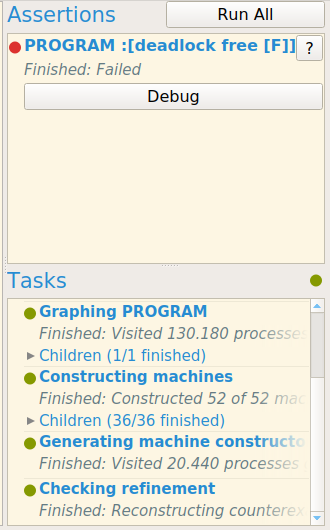
\includegraphics[height=10cm]{figuras/assertion.png}
\fonte{O autor}
\label{fig:assertion}
\end{figure}
%Iverson: adicionei esse paragrafo falando sobre um contraexemplo gerado apos a falha da verificacao no FDR
Como o resultado dessa verificação falhou o FDR exibe na interface um contraexemplo indicando o ponto no qual a falha aconteceu. A Figura \ref{fig:counterexem} apresenta o contraexemplo da verificação da propriedade \texttt{:[deadlock free [F]]} para o processo \texttt{PROGRAM}. Onde é possível ver a sequência de eventos comunicados no processo \texttt{COMMANDS}. Analisando os \textit{traces}, sabemos que esse processo comunicou o evento \texttt{right} inicialmente, seguido por cinco eventos \texttt{forward.1} e finalizou comunicando \texttt{showInt.2}, este mostra a quantidade de caixas à esquerda do robô, equivalente ao comando \texttt{show} em ROBO. Comparando com o programa ROBO descrito pela Figura \ref{fig:roboprogram} é possível notar que o último comando que o robô realizar é \texttt{show(counter)}.

\begin{figure}[h]
\centering
\caption{Contraexemplo gerado pelo FDR}
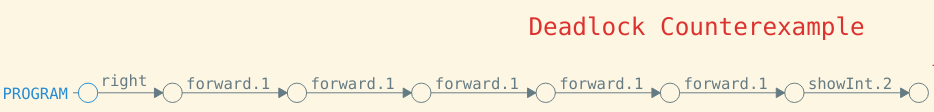
\includegraphics[height=2cm]{figuras/contraexe.png}
\fonte{O autor}
\label{fig:counterexem}
\end{figure}

%A ferramenta FDR ainda provê um \textit{feedback} visual da especificação dos sistemas. Está disposto na Figura \ref{fig:graph} parte da máquina de estados de um processo chamado \texttt{COMMANDS}. Cada estado representa um possível evento que possa ocorrer e em cada um deles há os possíveis outros estados que são acessíveis pelos os mesmos. Por exemplo, o evento inicial \texttt{right} pode dar origem a outros quatro eventos: \texttt{get.ORIENTATION.0}, \texttt{get.ORIENTATION.1}, \texttt{get.ORIENTATION.2} ou \texttt{get.ORIENTATION.3}.

%Diante disso, podemos afirmar que FDR de fato é uma ferramenta poderosa para esses tipos de verificações em cima de sistemas modelados em CSP, a fim de explorar possibilidades que o próprio sistema sozinho não fornece. 
Além da interface gráfica, FDR possui uma API (\textit{Application Programming Interface}) que permite o desenvolvimento de sistemas que usam os serviços de FDR. 

%\begin{figure}[h]
%\centering
%\caption{Máquina de estados de um processo CSP}
%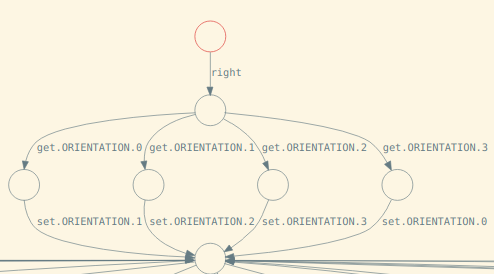
\includegraphics[height=7cm]{figuras/graph.png}
%\fonte{O autor}
%\label{fig:graph}
%\end{figure}

%\section{Processo de Compilação}
%\subsection{Linguagem de Domínio Específico - DSL}
%Uma Linguagem de Domínio Específico (\textit{Domain-Specific Language} - DSL) é uma linguagem que possui um propósito bem definido, diferente das linguagens de propósito geral como Java ou C. A criação de DSLs tem como característica a possibilidade de expressar soluções para problemas de modo mais claro que as linguagens de prepósito geral \cite{fowler}. A linguagem ROBO é um tipo de DSL que tem como finalidade a criação de programas para a simulação de robôs em um ambiente virtual. 

%A criação de um compilador para uma DSL depende do tipo da DSL. Geralmente para uma DSL interna, isto é, uma linguagem que é executada em cima de um compilador de uma linguagem de propósito geral, é necessário que a linguagem tenha o compilador modificado. Já para as DSLs externas, um novo compilador ou interpretador deve ser implementando \cite{schimitt}.


\section{Plataforma Spoofax}
\label{sec:compilacao}

Para criar um compilador da linguagem ROBO para CSP é necessário um mecanismo que ajude nesse processo. Neste trabalho vamos utilizar a Plataforma Spoofax.

Spoofax\footnote[6]{http://www.metaborg.org/} é uma plataforma para desenvolvimento textual de linguagens de programação. Esta plataforma permite o desenvolvimento através de um ambiente interativo usando metalinguagens (\textit{meta-languages)} para definição de linguagem declarativa de alto nível. Além disso, possui geradores de código que produzem analisadores (\textit{parses}), checagem de tipo, compiladores, interpretadores e outras ferramentas. A vantagem de usar Spoofax é o foco na essência da definição da linguagem, ignorando detalhes irrelevantes da implementação \cite{KatsSpoofax}.

Um projeto em Spoofax possui uma arquitetura muito bem estruturada, seguindo alguns princípios. Primeiro, separação de interesses, por exemplo, separa definição de sintaxe da definição da semântica estática. Segundo, não repete aspectos da linguagem em diferentes implementações, objetivando a geração de diferentes artefatos a partir de um único código. Por último, a definição de linguagem declarativa ocorre de modo independente, onde cada tipo de implementação possui sua própria linguagem correspondente. Por exemplo, para definição de sintaxe utiliza o formalismo SDF3, já para a parte de transformação, utiliza-se a metalinguagem Stratego \cite{KatsSpoofax}. Spoofax ainda provê outras metalinguagens, como por exemplo NaBL2, utilizada para a checagem semântica da linguagem, o que inclui checagem de nomes e análise de tipos. 

Para o escopo desse projeto, utilizamos SDF3 e Stratego, tendo em vista que a checagem de nomes e tipos da linguagem ROBO é realizada durante o desenvolvimento do programa dentro do ambiente RoboMind. 
% sidney : um aprimoramento futuro é fazer a verificação de tipos usando Spoofax, uma vez que na atual abordagem, deixamos que a verificação de tipos seja feita por FDR o que obriga o usuário da ferramenta de verificação entender de CSP para entender o problema do código ROBO

Assim como o verificador de modelos FDR, a plataforma Spoofax dispõe de uma API que pode ser utilizada para diferentes objetivos, como por exemplo, o desenvolvimento de ferramentas integradas a um compilador gerado pela plataforma.

\subsection{Definição Sintática com SDF3}

A definição sintática com Spoofax ocorre através da metalinguagem SDF3, esta é um formalismo que propicia a definição da sintaxe para linguagens de programação e Linguagem de Domínio Específico (\textit{Domain-Specific Language} - DSL). Na Figura \ref{fig:parsing} é mostrado o fluxograma de como ocorre a definição sintática com essa plataforma, desde a definição da gramática até a geração da árvore sintática. O primeiro passo é a definição dos módulos em SDF3, onde ocorre toda a definição da gramática da linguagem. Como saída dos módulos normalizados em SDF3, é gerada uma tabela de análise (\textit{Parse Table}) que é utilizado como entrada no \textit{Scannerless Generalized LR} (SGLR), responsável por produzir a Árvore de Sintaxe Abstrata (\textit{Abstract Syntax Tree} - AST). Após a geração de uma AST, o SDF3 conta com uma mecanismo que remove todas as ambiguidades, gerando uma única AST (\textit{Parse Tree}) de um programa em uma linguagem específica (\textit{Source Program}). 

\begin{figure}[h]
\centering
\caption{Processo de definição sintática do Spoofax}
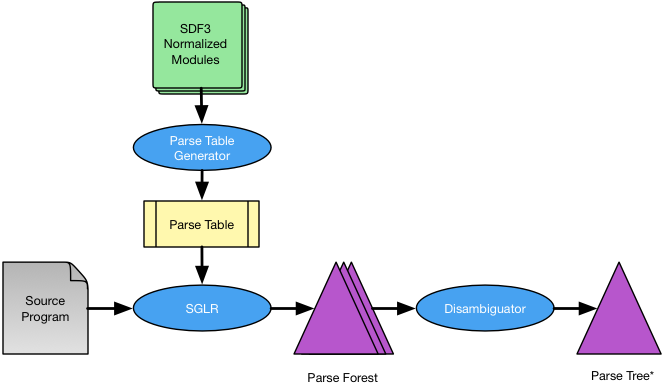
\includegraphics[height=7cm]{figuras/parsing.png}
\fonte{\cite{metaborg}}
\label{fig:parsing}
\end{figure}

A Figura \ref{fig:sdf} mostra como é a estrutura de um ambiente de programação utilizando essa metalinguagem. A parte mais a esquerda da figura mostra um exemplo da gramática de uma linguagem escrita no formado SDF3 (\textit{Example.sdf3}). Esse arquivo define um módulo (\texttt{module}) chamado \texttt{Example} que importa o módulo \texttt{Commons} e define a gramática a partir de quatro seções diferentes. 
%Todas essas seções da figura citada anteriormente são importantes para a definição final da gramática de uma linguagem. 
A seção \texttt{context-free start-symbols} indica os símbolos iniciais quando ocorre uma análise dos termos. A seção \texttt{context-free syntax} descreve em alto nível a estrutura sintática das sentenças em uma linguagem, contendo uma lista de produções. A seção \texttt{context-free priorities} é utilizado para remover ambiguidades através da definição de prioridades entre as produções. Por último, a seção \texttt{lexical syntax} descreve a parte léxica da linguagem, ou seja, como cada produção deve ser representada e também a definição de palavras reservadas da linguagem. O lado direito da Figura \ref{fig:sdf} mostra três diferentes arquivos. O quadrante superior é um editor com \textit{syntax highlighting} que é produzido automaticamente pelo ambiente a partir da definição da gramática SDF3. Além da marcação da sintaxe, este editor possui \textit{auto complete} dos termos da linguagem.
%No quadrante de cima, mostra como é a interação durante uma codificação de um programa na linguagem definida, mostrando sugestões da gramática. 
O quadro do meio mostra um exemplo de código aceito pela gramática. O último quadro (\textit{Example.aterm}) mostra a árvore sintática do programa \textit{Example.tes}.


\begin{figure}[h]
\centering
\caption{Definição sintática com SDF3}
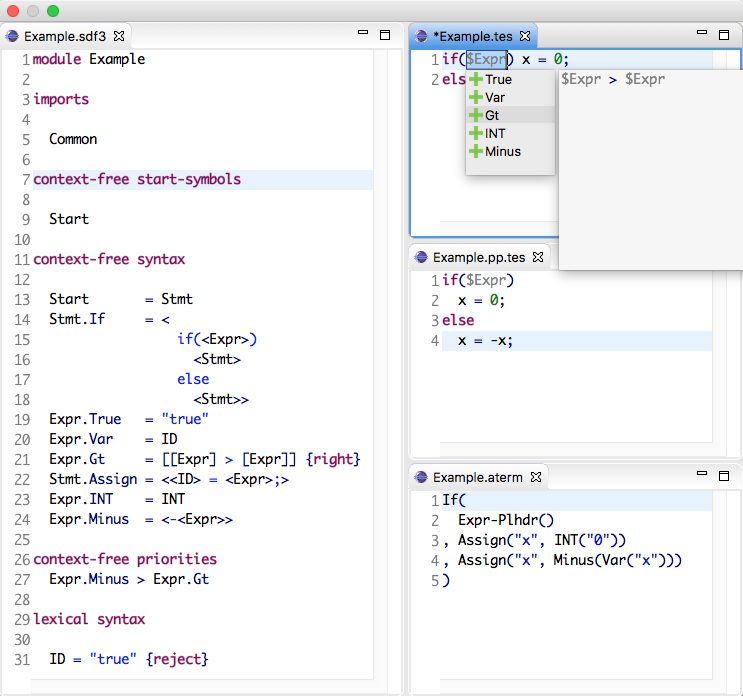
\includegraphics[height=10cm]{figuras/sdf3-spoofax.png}
\fonte{\cite{metaborg}}
\label{fig:sdf}
\end{figure}

A definição sintática com Spoofax, mais especificamente usando a metalinguagem SDF3
%, como visto, ocorre de modo alto nível, facilitando todo esse processo. Como 
produz uma árvore sintática não ambígua que é essencial para a etapa seguinte do processo de compilação, a geração de código. A transformação ocorre através da metalinguagem Stratego.

\subsection{Transformação com Stratego}

%A transformação de programas nada mais é do que manipulação mecânica de um programa com a finalidade de melhorar seu custo computacional. Exemplo, seja $C(P)$ uma função, então aplicamos uma transformação em $P$, logo temos $C(P) > C(tr(P))$, ou seja o custo computacional da função transformada é inferior à função original \cite{metaborg}. Sabendo disso, temos a consciência da importância das transformações em um processo de compilação. 

Este projeto usa Stratego para traduzir automaticamente o código ROBO em CSP com finalidade de analisar automaticamente a corretude dos programas ROBO. Stratego é usado para definir a regra de transformação cada elemento sintático de ROBO para a respectiva representação em CSP.

Stratego é uma metalinguagem para a definição de transformações aplicadas à uma AST. Essa metalinguagem tem uma notação capaz de construir e descontruir a árvore e usar reescrita de termos (\textit{term rewriting}), que basicamente reestrutura a árvore ou utiliza termos de interesse em uma determinada transformação. Essas transformações ocorrem em decorrência da definição de regras e estratégias. Os elementos da AST são representados por termos, como mostrado no arquivo \textit{Example.aterm} da Figura \ref{fig:sdf}. Esses termos estão na notação chamada de Formato de Termo Anotado (\textit{Annotated Term Format} - ATerm), uma notação que facilita a manipulação da árvore pelo Stratego  \cite{metaborg}. Por exemplo, em ROBO o comando \texttt{forward(n)} é denotado em \textit{ATerm} por \texttt{Instr(FORWARD(Var("n")))}.

Uma regra em Stratego é definida como uma transformação aplicada em um ou mais termos. Uma regra é dada por \texttt{L : p1 -> p2}, onde \texttt{L} é o nome da regra, \texttt{p1} é o termo que deve casar com a regra e \texttt{p2} o termo reescrito. Como alternativa, a saída de uma regra pode ser textual, ao invés de um termo reescrito. Esta abordagem é chamada interpolação de \textit{string} \cite{KatsSpoofax}. Uma regra desse tipo é dada por \texttt{L : T(p) -> \$[[p]]}, no qual \texttt{L} é o nome da regra, \texttt{T(p)} o termo que deve casar com a regra, e o texto na linguagem destino é gerado com o conteúdo entre \texttt{\$[} e \texttt{]} utilizando o valor de \texttt{p}. Além disso, é possível aplicar outras regras a partir de \texttt{p} utilizando a palavra reservada \texttt{with} no fim da regra. As regras definidas em~\cite{nogueira} para mapear a AST de programas ROBO para CSP utiliza interpolação de \textit{strings}. As \textit{strings} produzidas como resultado da regra correspondem ao modelo CSP para o programa ROBO representado pela AST de entrada. Isso é demonstrado em detalhes na Seção \ref{chap:cap3}. 

% sidney: não precisa falar de conceitos que não são utilizados no trabalho
%É importante saber que as estratégias são combinações de uma ou mais transformações dentro de uma nova transformação, elas são mais utilizadas para a remoção de tautologias e preposições falsas nos termos \cite{KatsSpoofax}. Para esta pesquisa, as estratégias não são muito relevantes, uma vez que o foco estão na definição de regras e eventualmente são utilizadas.

O Stratego possui algumas funções que podem ser utilizadas durante uma transformação. Por exemplo, há algumas funções que são usadas para filtrar termos em uma AST, ou seja, apenas termos de interesse são aplicados em uma transformação. É o caso da função \texttt{filter} que retorna uma lista com o conjunto de termos filtrados, esse filtro é aplicado apenas aos termos que estão no primeiro nível da árvore. Outra função importante é \texttt{collect-all}, que é responsável por recolher todos os termos em uma AST que casem com o termo analisado, essa busca ocorre em todos os níveis da árvore.

%Esses conceitos são extremamente importantes para acompanhar o raciocínio desenvolvido no próximo capítulo, em virtude de que é apresentado na prática diferentes definições de regras, com intuito de gerar a notação CSP para variáveis e procedimentos da linguagem ROBO.